\chapter{Ristrutturazione e traduzione dello schema}
In questo capitolo procederemo alla preparazione dello schema per poi tradurlo direttamente in uno schema relazionale per PostgreSQL, specificando anche delle soluzioni per
rispettare i vincoli esterni definiti.
\section{Ristrutturazione dello schema Entity-Relationship}
Procediamo alla ristrutturazione dello schema ER prima di tradurlo direttamente nello schema relazionale:
\begin{itemize}
  \item Sostituiamo le relationship Molti a Molti, tipicamente introducendo una nuova tabella
  \item Sostituiamo eventuali relazioni is-a.
  \item Selezioniamo o introduciamo le chiavi primarie.
  \item Aggiungiamo in modo controllato della ridondanza, se necessario per questioni di performance (Es. un campo precalcolato in caso di accessi frequenti a un dato derivato).
  \item Introduciamo ulteriori vincoli esterni in seguito alla ristrutturazione, se lo schema ristrutturato non rispetta pi\`u i vincoli dello schema originale.
\end{itemize}
\begin{figure}[H]
  \centering
  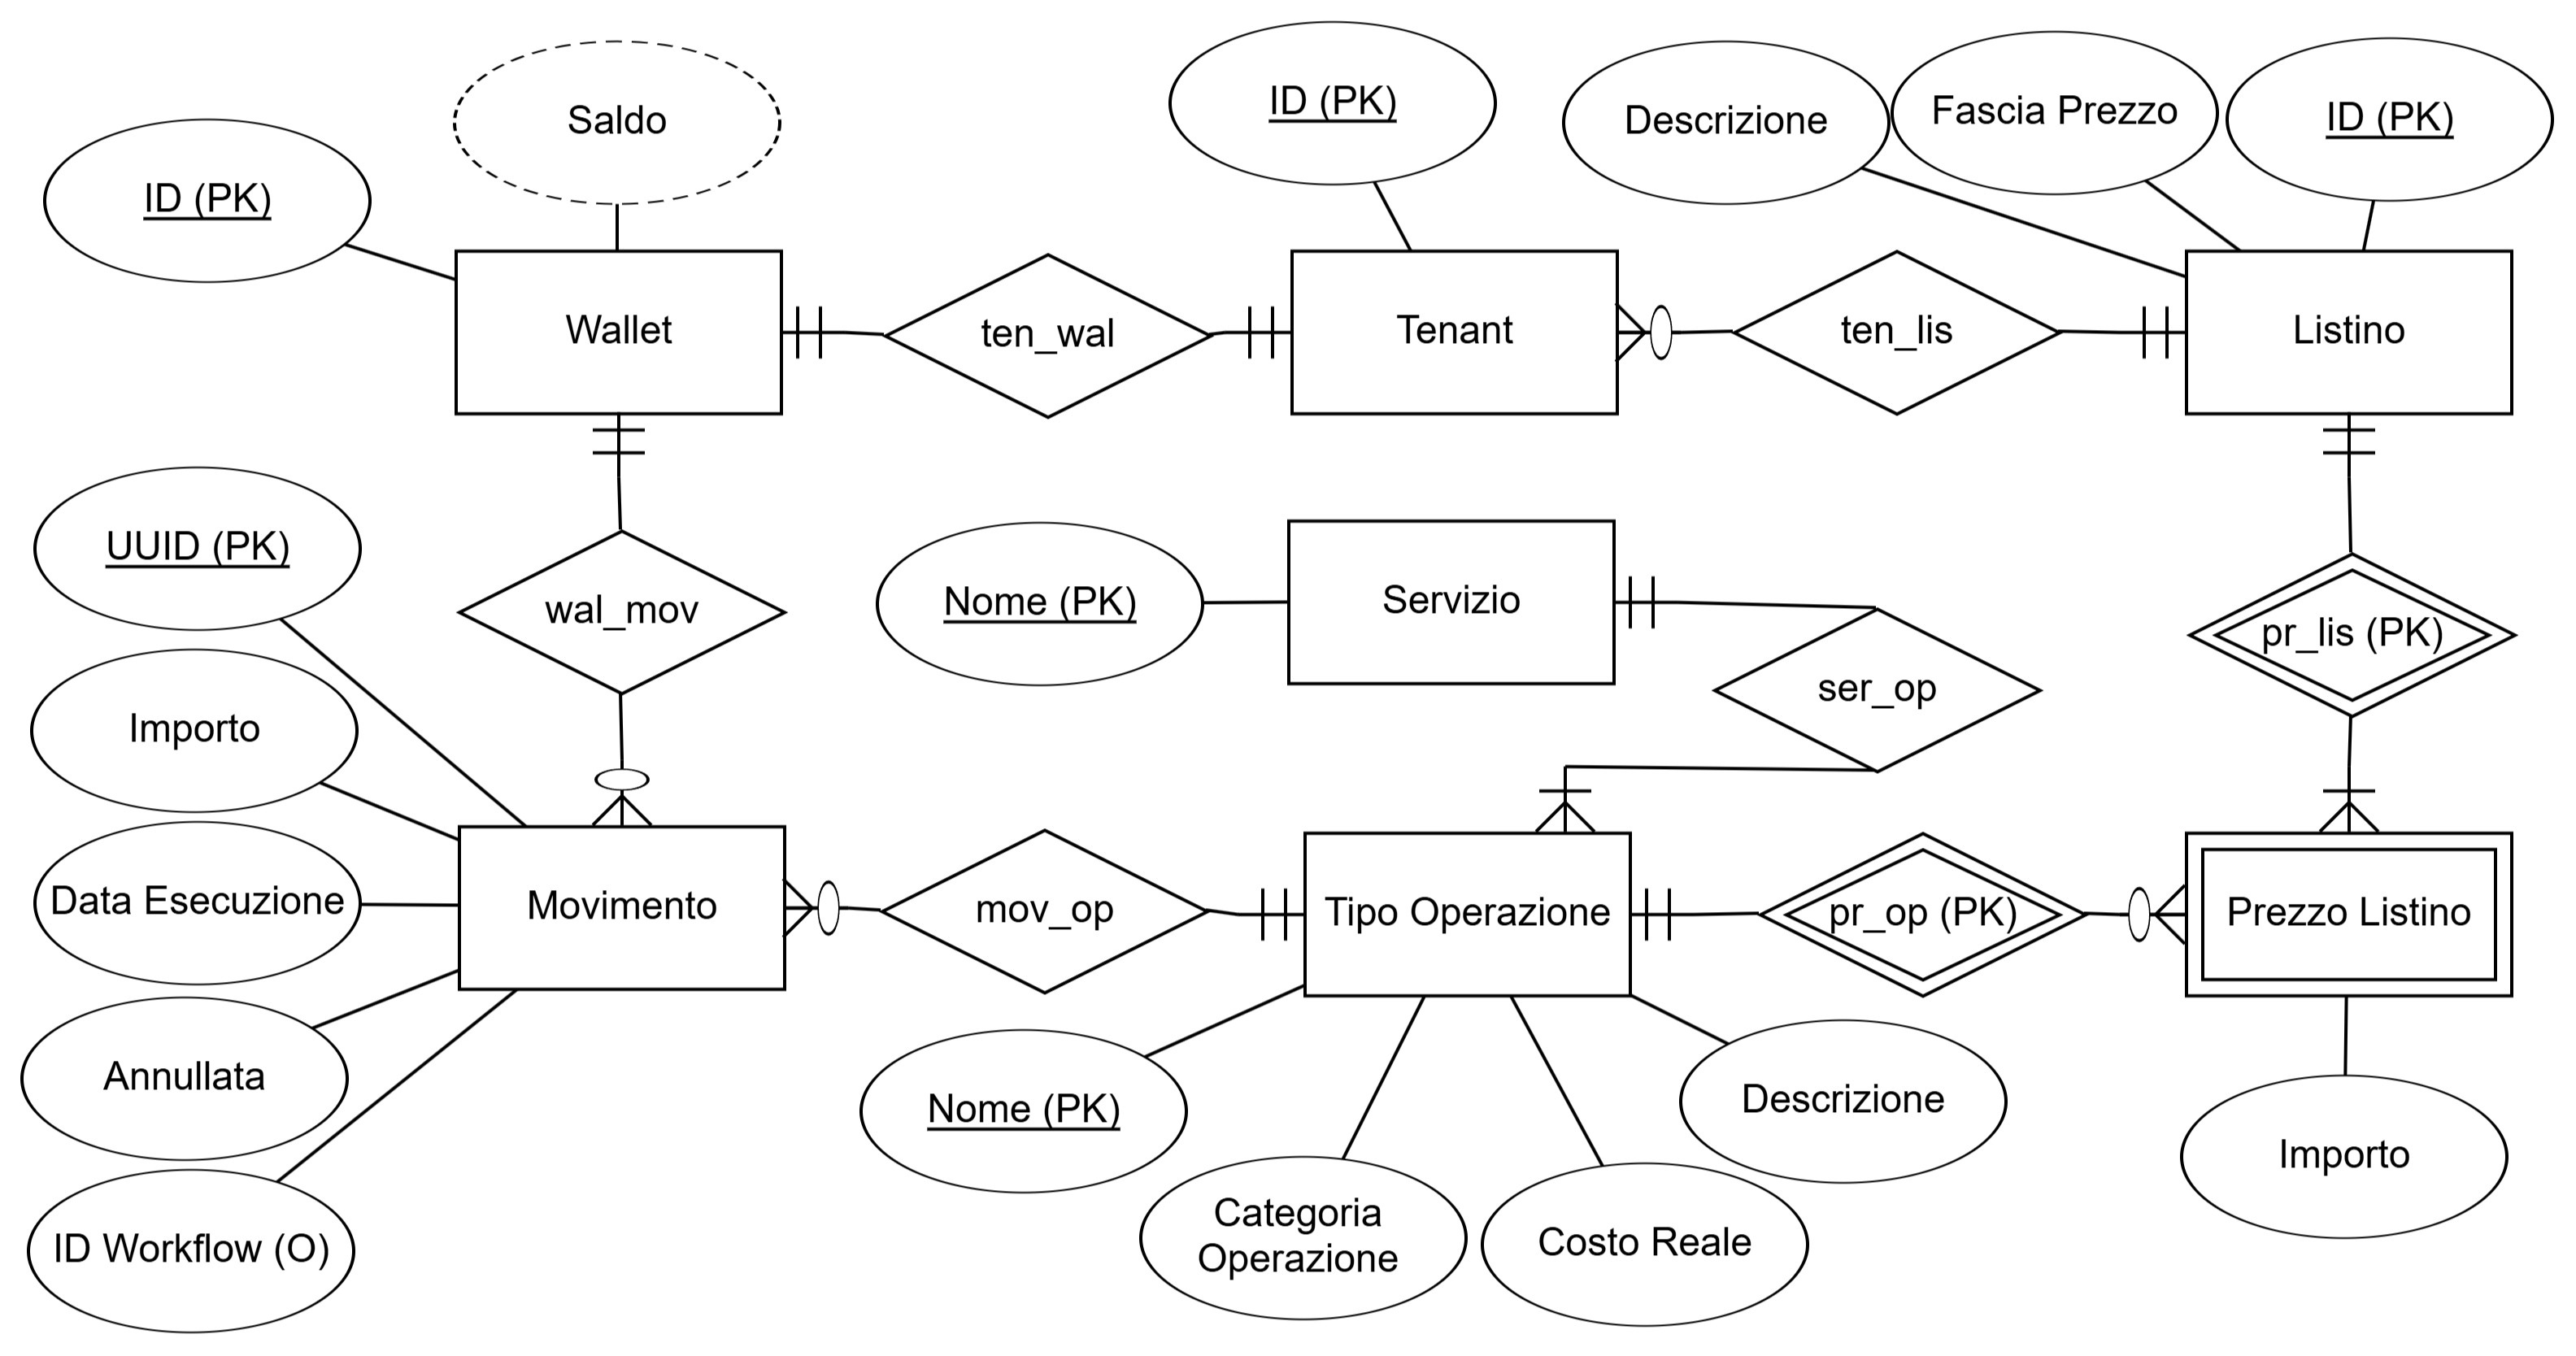
\includegraphics[width=13cm]{images/db-diagrams/er-diagram-ristrutturato.png}
  \caption{Schema Entity-Relationship tradotto}
\end{figure}

\section{Traduzione dello schema ristrutturato}
Traduciamo lo schema ristrutturato nello schema relazionale da inserire in PostgreSQL, con chiavi primarie e chiavi esterne.

\textbf{Movimento(\underline{uuid}, importo, dataEsecuzione, descrizione, idWorkflow*,\\ tipoOperazioneId, walletId) \\}
\textbf{\hspace*{1.5 cm} foreign key: $ Movimento[tipoOperazioneId] \subseteq TipoOperazione[nome] $} \\
\textbf{\hspace*{1.5 cm} foreign key: $ Movimento[walletId] \subseteq Wallet[id] $ }
\\\\
\textbf{TipoOperazione(\underline{nome}, servizio, categoriaOperazione, costoReale, \\descrizione) \\}
\textbf{\hspace*{1.5 cm} foreign key: $ TipoOperazione[servizio] \subseteq Servizio[nome] $}
\\\\
\textbf{Servizio(\underline{nome})}
\\\\
\textbf{Wallet(\underline{id}, saldo, tenantId) \\}
\textbf{\hspace*{1.5 cm} key:} \textit{(tenantId)} \\
\textbf{\hspace*{1.5 cm} foreign key: $ Wallet[tenantId] \subseteq Tenant[id] $}
\\\\
\textbf{Tenant(\underline{id}, listinoId) \\}
\textbf{\hspace*{1.5 cm} foreign key: $ Tenant[listinoId] \subseteq Listino[id] $}
\\\\
\textbf{Listino(\underline{id}, descrizione, fasciaPrezzo)}
\\\\
\textbf{PrezzoListino(\underline{tipoOperazioneId}, \underline{listinoId}, importo) \\}
\textbf{\hspace*{1.5 cm} foreign key: $ PrezzoListino[tipoOperazioneId] \subseteq TipoOperazione[nome] $} \\
\textbf{\hspace*{1.5 cm} foreign key: $ PrezzoListino[listinoId] \subseteq Listino[id] $}

\begin{figure}[H]
  \centering
  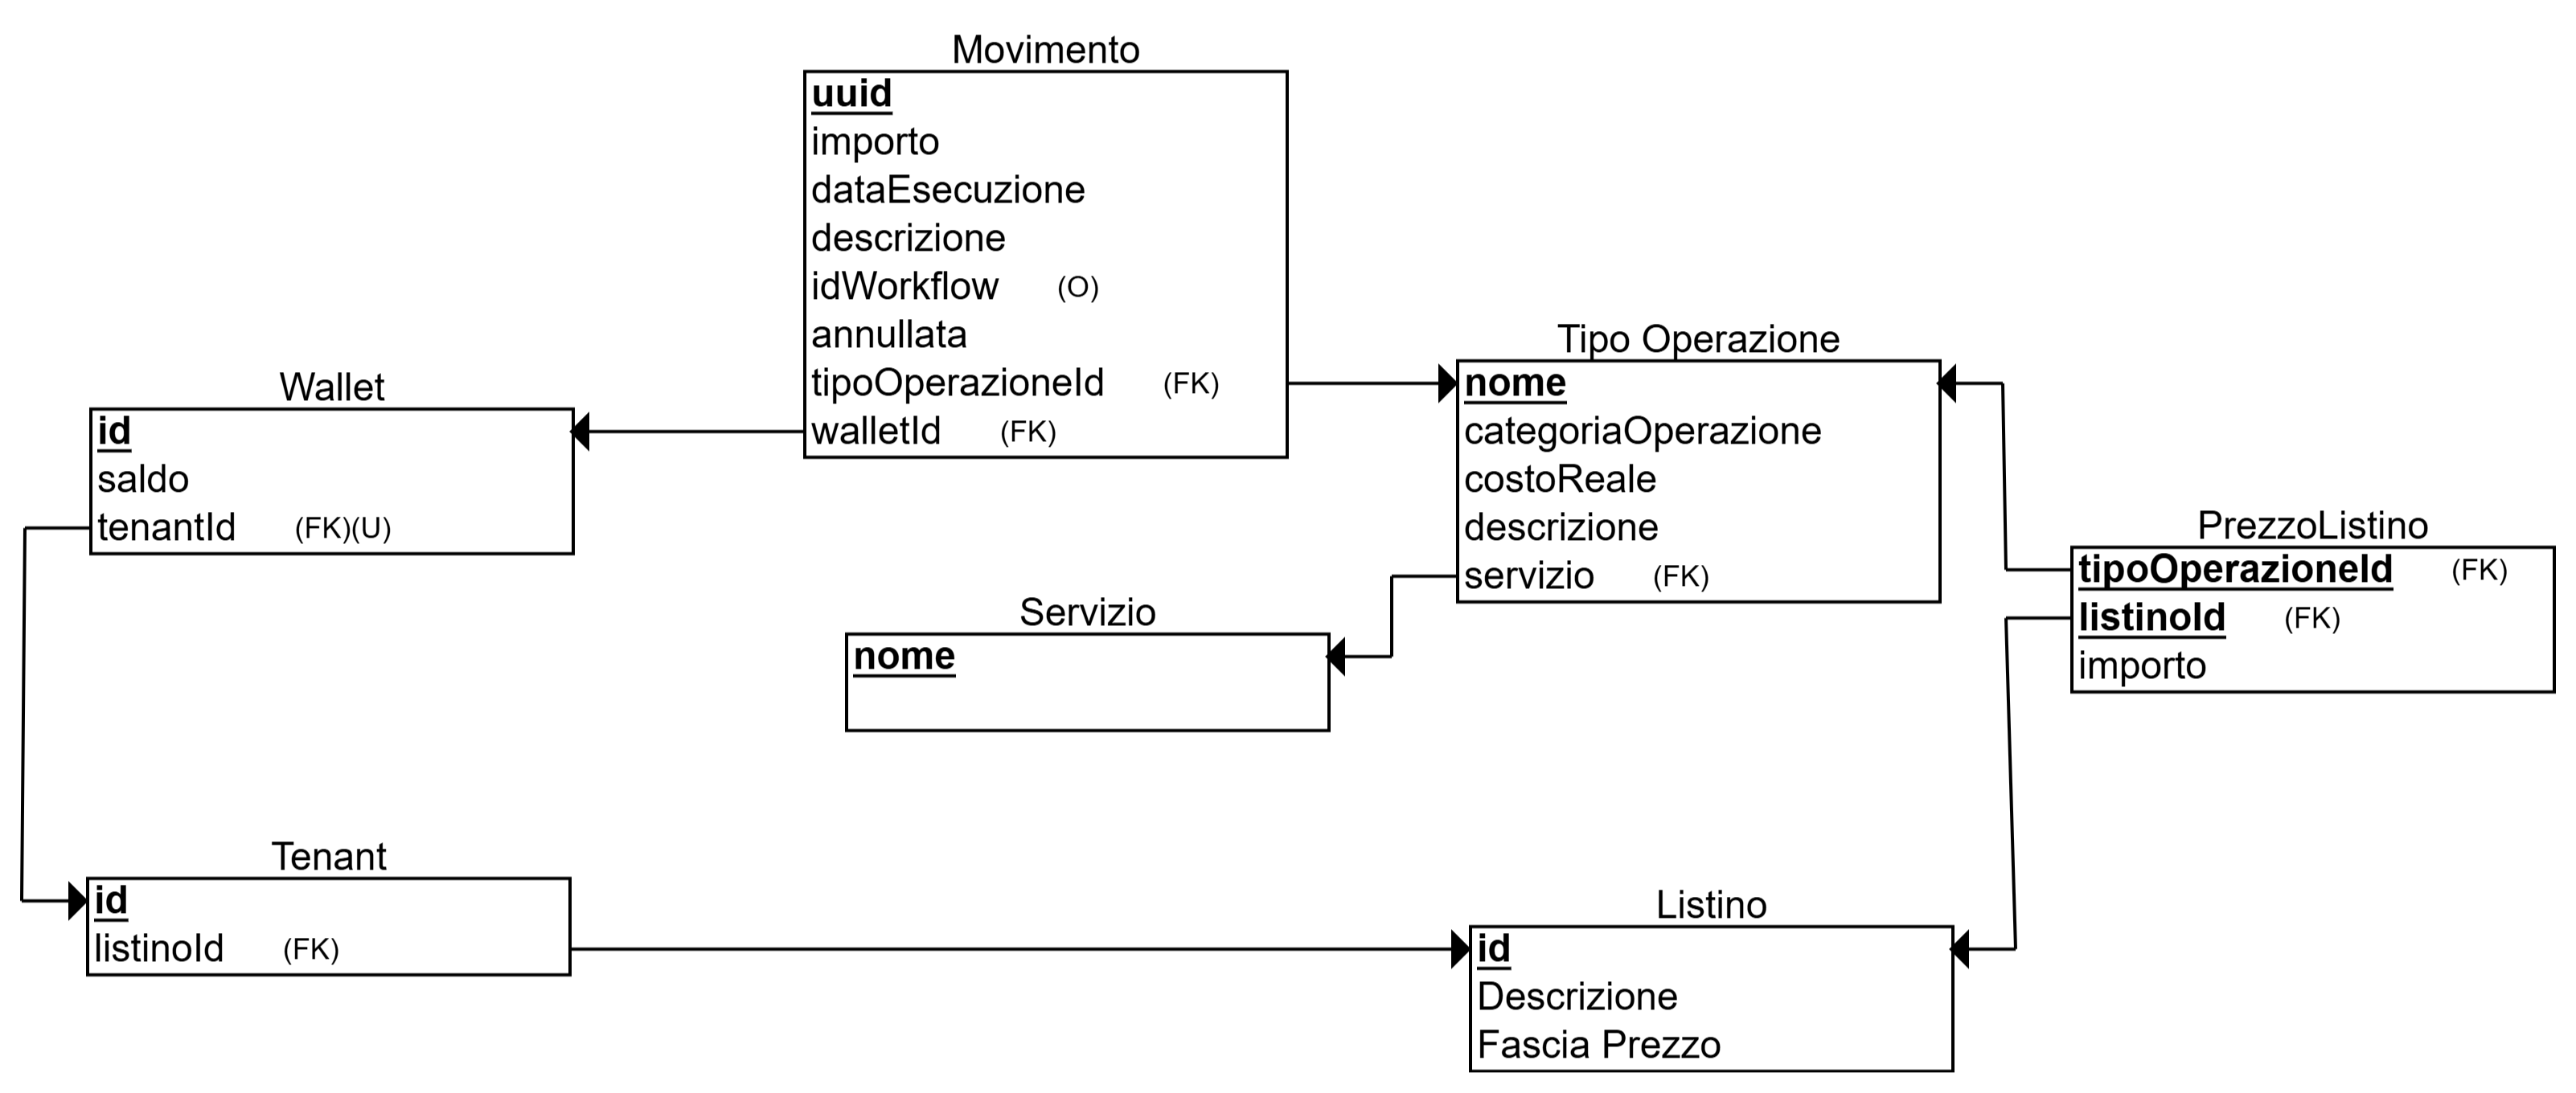
\includegraphics[width=13cm]{images/db-diagrams/rappresentazione-grafica-db.png}
  \caption{Rappresentazione grafica del database}
\end{figure}

\section{Traduzione dei vincoli esterni}
Visto che non sono stati aggiunti ulteriori vincoli esterni durante la ristrutturazione, occupiamoci dell'unico vincolo che \`e stato riconosciuto durante
la creazione dello schema concettuale:
\\\\
\textbf{Tutti gli importi specificati (\ref{tuttiimporticoncept})} - Come vedremo nel prossimo capitolo \textbf{(\ref{designinserimentoprezzi})}, il vincolo verr\`a forzato dal form di creazione.

\section {Tabelle pre-popolate}
Ci sono due tabelle di cui conosciamo il contenuto a priori, e che non \`e possibile modificare da interfaccia: TipoOperazione e Servizio. Pertanto, inseriremo dei dati per popolarle
durante l'inizializzazione del database.
